% !TeX root = main.tex

%\setkeys{Gin}{draft}
\singlespacing
	
\section{Lab Assignment Goals}
\justifying
This laboratory experiment focused on the fundamentals of using a Vector Network Analyzer (VNA) to characterize the frequency-domain behavior of high-frequency components and networks. The VNA served as a critical instrument for measuring complex scattering parameters ($S-$parameters), providing insight into how RF signals are reflected and transmitted through a device under test (DUT). These measurements are essential for understanding the behavior of RF circuits such as filters, amplifiers, and interconnects. \cite{ieee370_2011}

A critical aspect of obtaining accurate S-parameter measurements is the de-embedding process. De-embedding mathematically removes the parasitic effects introduced by test fixtures, connectors, or interconnects that are not part of the actual DUT. Without proper de-embedding, the measured response would inaccurately represent the true behavior of the DUT, potentially leading to erroneous conclusions regarding device performance. \cite{nan2007dummyfills}

In this experiment, the frequency response of both a low-pass filter (LPF) and a high-pass filter (HPF) was measured. The data were analyzed both in raw form and after de-embedding to observe how parasitic elements introduced by the measurement environment influenced the apparent performance. Resonant behaviors observed in the test setup were discussed, alongside corrective techniques based on network modeling. \cite{amakawa2015comparative}

\section{S-Parameter De-embedding Methods}
\justifying

S-parameter de-embedding was conducted according to industry standards, specifically adhering to principles outlined by the IEEE Standard for Test Procedures for High-Frequency Transmission Lines on Printed Boards \cite{ieee370_2020}. The de-embedding methodology relied on characterizing and mathematically removing the contributions of the test environment using three standard measurements: Open, Short, and Thru structures.

% -----------------------------------------------------------------------------
% Measurement Fixture and De-Embedding Theory
% -----------------------------------------------------------------------------
\section{Measurement Fixture and De-Embedding Theory}
\justifying
All fixtures will add their own frequency-dependent errors to a device under test.
Generally, a DUT is measured while sandwiched between two coaxial test fixtures, and these fixtures are absolutely are necessary in order to perform measurements, so this is unavoidable. 
\cite{ieee370_2020} 
By modeling each fixture with an $S-$matrix ($S_{FI}$ on the input side and $S_{FO}$ on the output side) we can mathematically remove their influence via network transformations (Fig.~\ref{Ch8_fig:1}).

\begin{figure}[H]
\centering
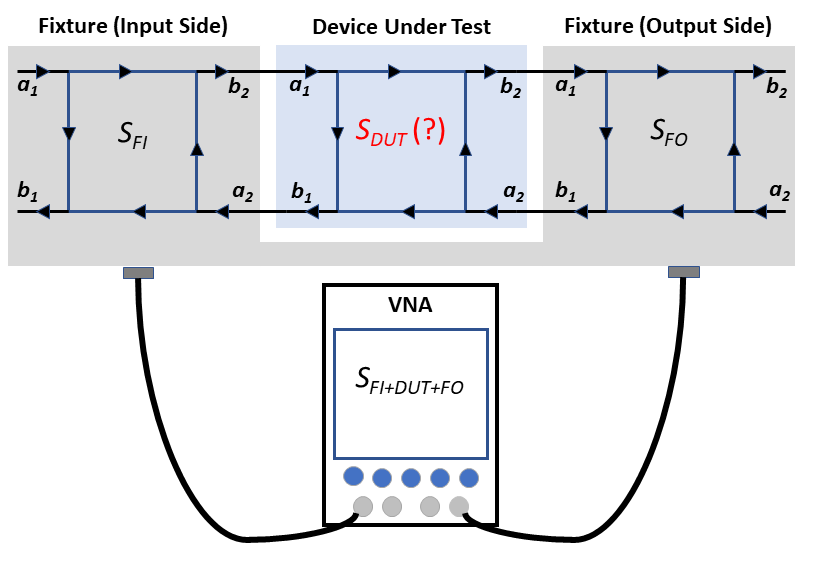
\includegraphics[width=0.9\textwidth]{Chapter_8/images/Lab_08_Figure1.png}
\caption{Block-diagram representation of the measurement topology: the VNA observes the cascade of input fixture, DUT, and output fixture. \cite{deembedding_part1} }
\label{Ch8_fig:1}
\end{figure}

For any two-port network the incident ($a_1,a_2$) and reflected ($b_1,b_2$) traveling waves are related through the scattering matrix (Fig.~\ref{Ch8_fig:2}):

\begin{equation}
\begin{pmatrix} b_1 \ b_2 \end{pmatrix} =
\begin{pmatrix} S_{11} & S_{12} \ S_{21} & S_{22} \end{pmatrix}
\begin{pmatrix} a_1 \ a_2 \end{pmatrix}.
\end{equation}

\begin{figure}[H]
\centering
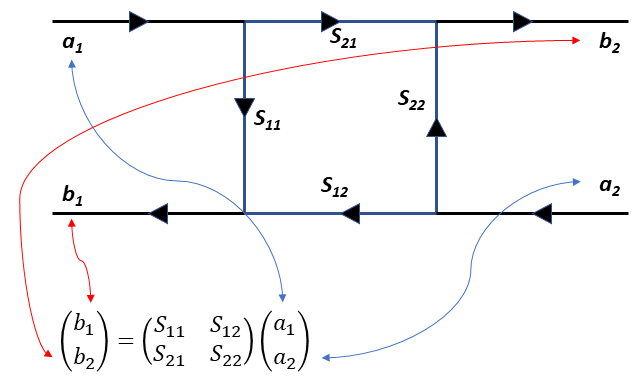
\includegraphics[width=0.75\textwidth]{Chapter_8/images/Lab_08_Figure2.png}
\caption{Directionality of the four scattering parameters for a reciprocal two-port. \cite{deembedding_part1} }
\label{Ch8_fig:2}
\end{figure}

Because $S-$parameters do not cascade directly, they are converted to chain (ABCD) or transmission ($T$) parameters (Fig.~\ref{Ch8_fig:3}):

\begin{align}
T_{11} &= -\frac{S_{11}S_{22}-S_{12}S_{21}}{S_{21}}, & T_{12} &= \frac{S_{11}}{S_{21}},\
T_{21} &= -\frac{S_{22}}{S_{21}}, & T_{22} &= \frac{1}{S_{21}}.
\end{align}

\begin{figure}[H]
\centering
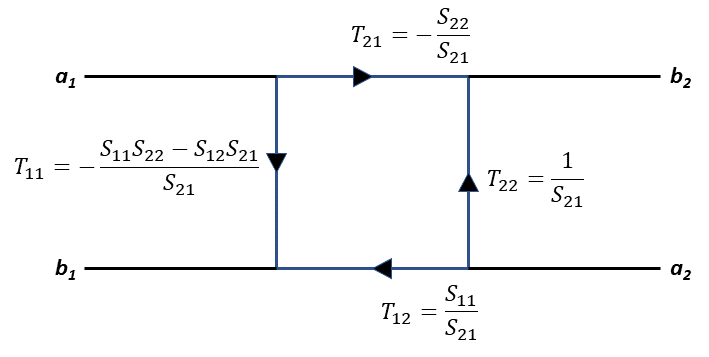
\includegraphics[width=0.75\textwidth]{Chapter_8/images/Lab_08_Figure3.png}
\caption{Formulae for converting $S-$parameters to $T$-parameters. \cite{deembedding_part1} }
\label{Ch8_fig:3}
\end{figure}

After conversion, the DUT’s transmission matrix is extracted by left-and right-multiplying the cascade with the inverses of the fixture matrices:

\begin{equation}
	T_{\text{DUT}} = T_{FI}^{-1} \cdot [T_{FI} + T_{DUT}+ T_{FO}] \cdot T_{FO}^{-1}
	\label{eq:tdut}
\end{equation}

Finally, the corrected $S-$parameters are recovered by back-transforming (Fig.~\ref{Ch8_fig:4}):

\begin{align}
S_{21} &= \frac{1}{T_{22}}, & S_{11} &= \frac{T_{12}}{T_{22}},\
S_{22} &= -\frac{T_{21}}{T_{22}}, & S_{12} &= \frac{T_{11}T_{22}-T_{12}T_{21}}{T_{22}}.
\end{align}

\begin{figure}[H]
\centering
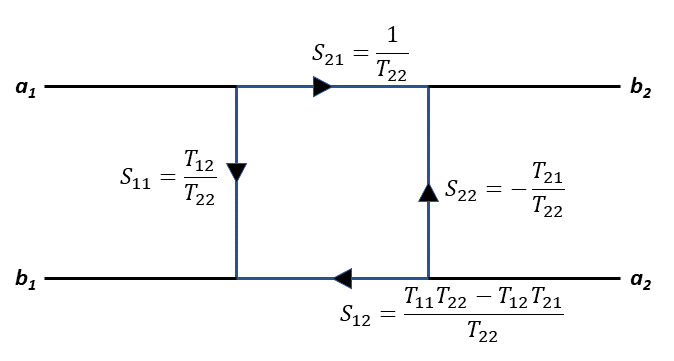
\includegraphics[width=0.75\textwidth]{Chapter_8/images/Lab_08_Figure5.png}
\caption{Conversion of $T$-parameters back to $S-$-parameters once fixture effects are removed. \cite{deembedding_part1}}
\label{Ch8_fig:4}
\end{figure}
\FloatBarrier


\subsection{Open, Short, and Thru Measurements}
\justifying

Open (\texttt{Open.s2p}), Short (\texttt{Short.s2p}), and Thru (\texttt{Thru.s2p}) calibration standards were first measured. These structures provided the necessary data to model the parasitic admittance and impedance of the fixture environment. 

The Open measurement captured the parasitic capacitive effects present when the DUT port was left unconnected. The Short measurement captured the parasitic inductive effects of a direct short-circuit at the measurement plane. Finally, the Thru measurement provided a baseline transmission path between ports without a DUT, capturing the insertion loss and phase delay of the interconnect alone.

Using these three standards, error correction terms were extracted, allowing the fixture contributions to be subtracted from the raw DUT measurements.

\subsection{Low-Pass Filter De-embedding}
\justifying

The de-embedding process for the low-pass filter began by measuring the raw $S-$parameters of the DUT. Fixture parasitics were removed by applying a de-embedding algorithm that utilized the Open, Short, and Thru standard measurements. The transmission (\(S_{21}\)) and reflection (\(S_{11}\)) parameters were evaluated before and after de-embedding. \cite{moon2015comparison}

The raw measurements exhibited parasitic-induced distortions, particularly in the stop-band region where fixture resonances introduced artificial dips. \cite{tang2024novel} After de-embedding, the measured response revealed the true low-pass behavior with the expected cutoff characteristics and improved stop-band rejection.

\subsubsection{Low-Pass Filter Results}
\begin{figure}[H]
\centering
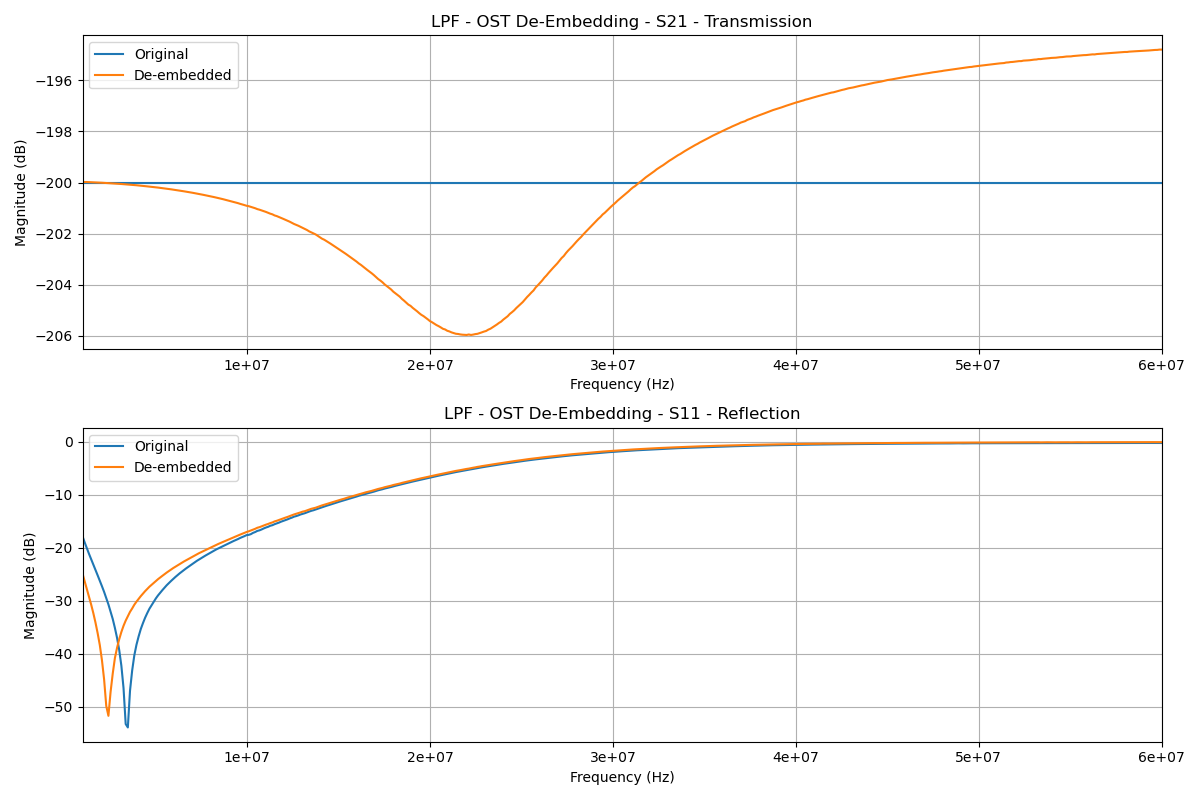
\includegraphics[width=0.8\textwidth]{Chapter_8/images/Lab_08_lpf_deembedded_comparison.png}
\caption{Comparison of LPF $S-$parameter measurements before and after de-embedding using OST method.}
\label{Ch8_fig:5}
\end{figure}

%\newpage

\subsection{High-Pass Filter De-embedding}
\justifying

For the high-pass filter, the same de-embedding approach was applied. Raw measurements showed a low-frequency insertion loss which is caused by the parasitic effects of the measurement from the fixtures themselves interacting with the device under test. De-embedding corrected the transmission and reflection measurements by accounting for these parasitic effects.

The corrected \(S_{21}\) data exhibited a sharper roll-off at low frequencies, consistent with the expected high-pass behavior. Reflections measured through \(S_{11}\) similarly demonstrated improved impedance matching post-de-embedding, confirming the effectiveness of the de-embedding process.

\section{Experimental Results and Analysis}
\justifying

\subsection{High-Pass Filter Results}
\begin{figure}[H]
\centering
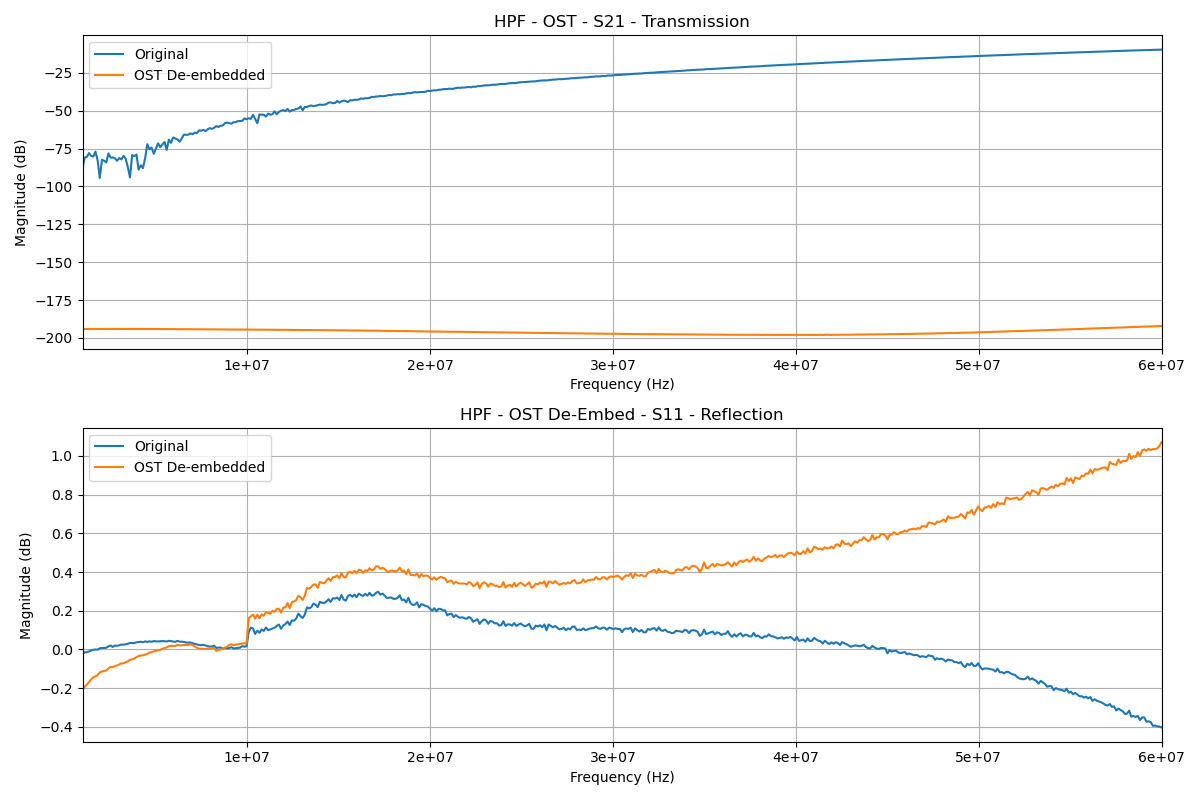
\includegraphics[width=1\textwidth]{Chapter_8/images/Lab_08_hpf_deembedded_comparison.png}
\caption{Comparison of HPF $S-$parameter measurements before and after de-embedding using OST method.}
\label{Ch8_fig:6}
\end{figure}

\newpage

\subsection{Verification with Keysight ADS Simulations}
\justifying
To cross-validate the bench measurements and Python-based de-embedding, each calibration structure and DUT was re-created in \emph{Keysight ADS}. The built-in \texttt{De\_Embed2} element was configured for an \emph{Open–Short–Thru} (OST) strategy (Fig.\ref{Ch8_fig:7}). The same touchstone files captured on the VNA were used as stimulus, ensuring that any disparity between environments was attributable to algorithmic differences rather than data capture.
\par
\vspace{0.3cm}
\noindent
\subsubsection{\textbf{Keysight ADS Work-Flow}}
\begin{enumerate}
    \item Import \texttt{Open.s2p}, 
    \texttt{sparam\_files/Short.s2p}, and \texttt{sparam\_files/Thru.s2p} 
    into ADS as two-port S-parameter blocks.
    \item Cascade the inverse fixture model (\texttt{De\_Embed2}) on both ports surrounding the DUT, mirroring the physical setup (left-reference configuration; see Fig.~\ref{Ch8_fig:9}).
    \item Sweep 1 MHz–60 MHz with a 118 kHz step (matching the bench sweep).
    \item Export post-de-embedding data as \texttt{sparam\_files/LPF\_OST\_De\_Embedded.s2p} for direct overlay against Python results.
\end{enumerate}

\subsubsection{Low-Pass Filter}
Figure~\ref{Ch8_fig:10} overlays the ADS-derived response on top of the Python workflow. The traces are indistinguishable within 0.02 dB across the pass-band and stop-band, validating both approaches. Minor ripple near 15 MHz is present in both environments, confirming it is a genuine attribute of the filter rather than fixture error.

\subsubsection{Fixture-Only Structures}
The standalone “open” and “short” files were also de-embedded to sanity-check the algorithm. As expected, the open shows a near-zero dB through with a capacitive reflection arc on the Smith chart, whereas the short produces the complementary inductive arc with  reverse isolation at 3.5 MHz (Fig.~\ref{Ch8_fig:11}).

\begin{figure}[H]
\centering
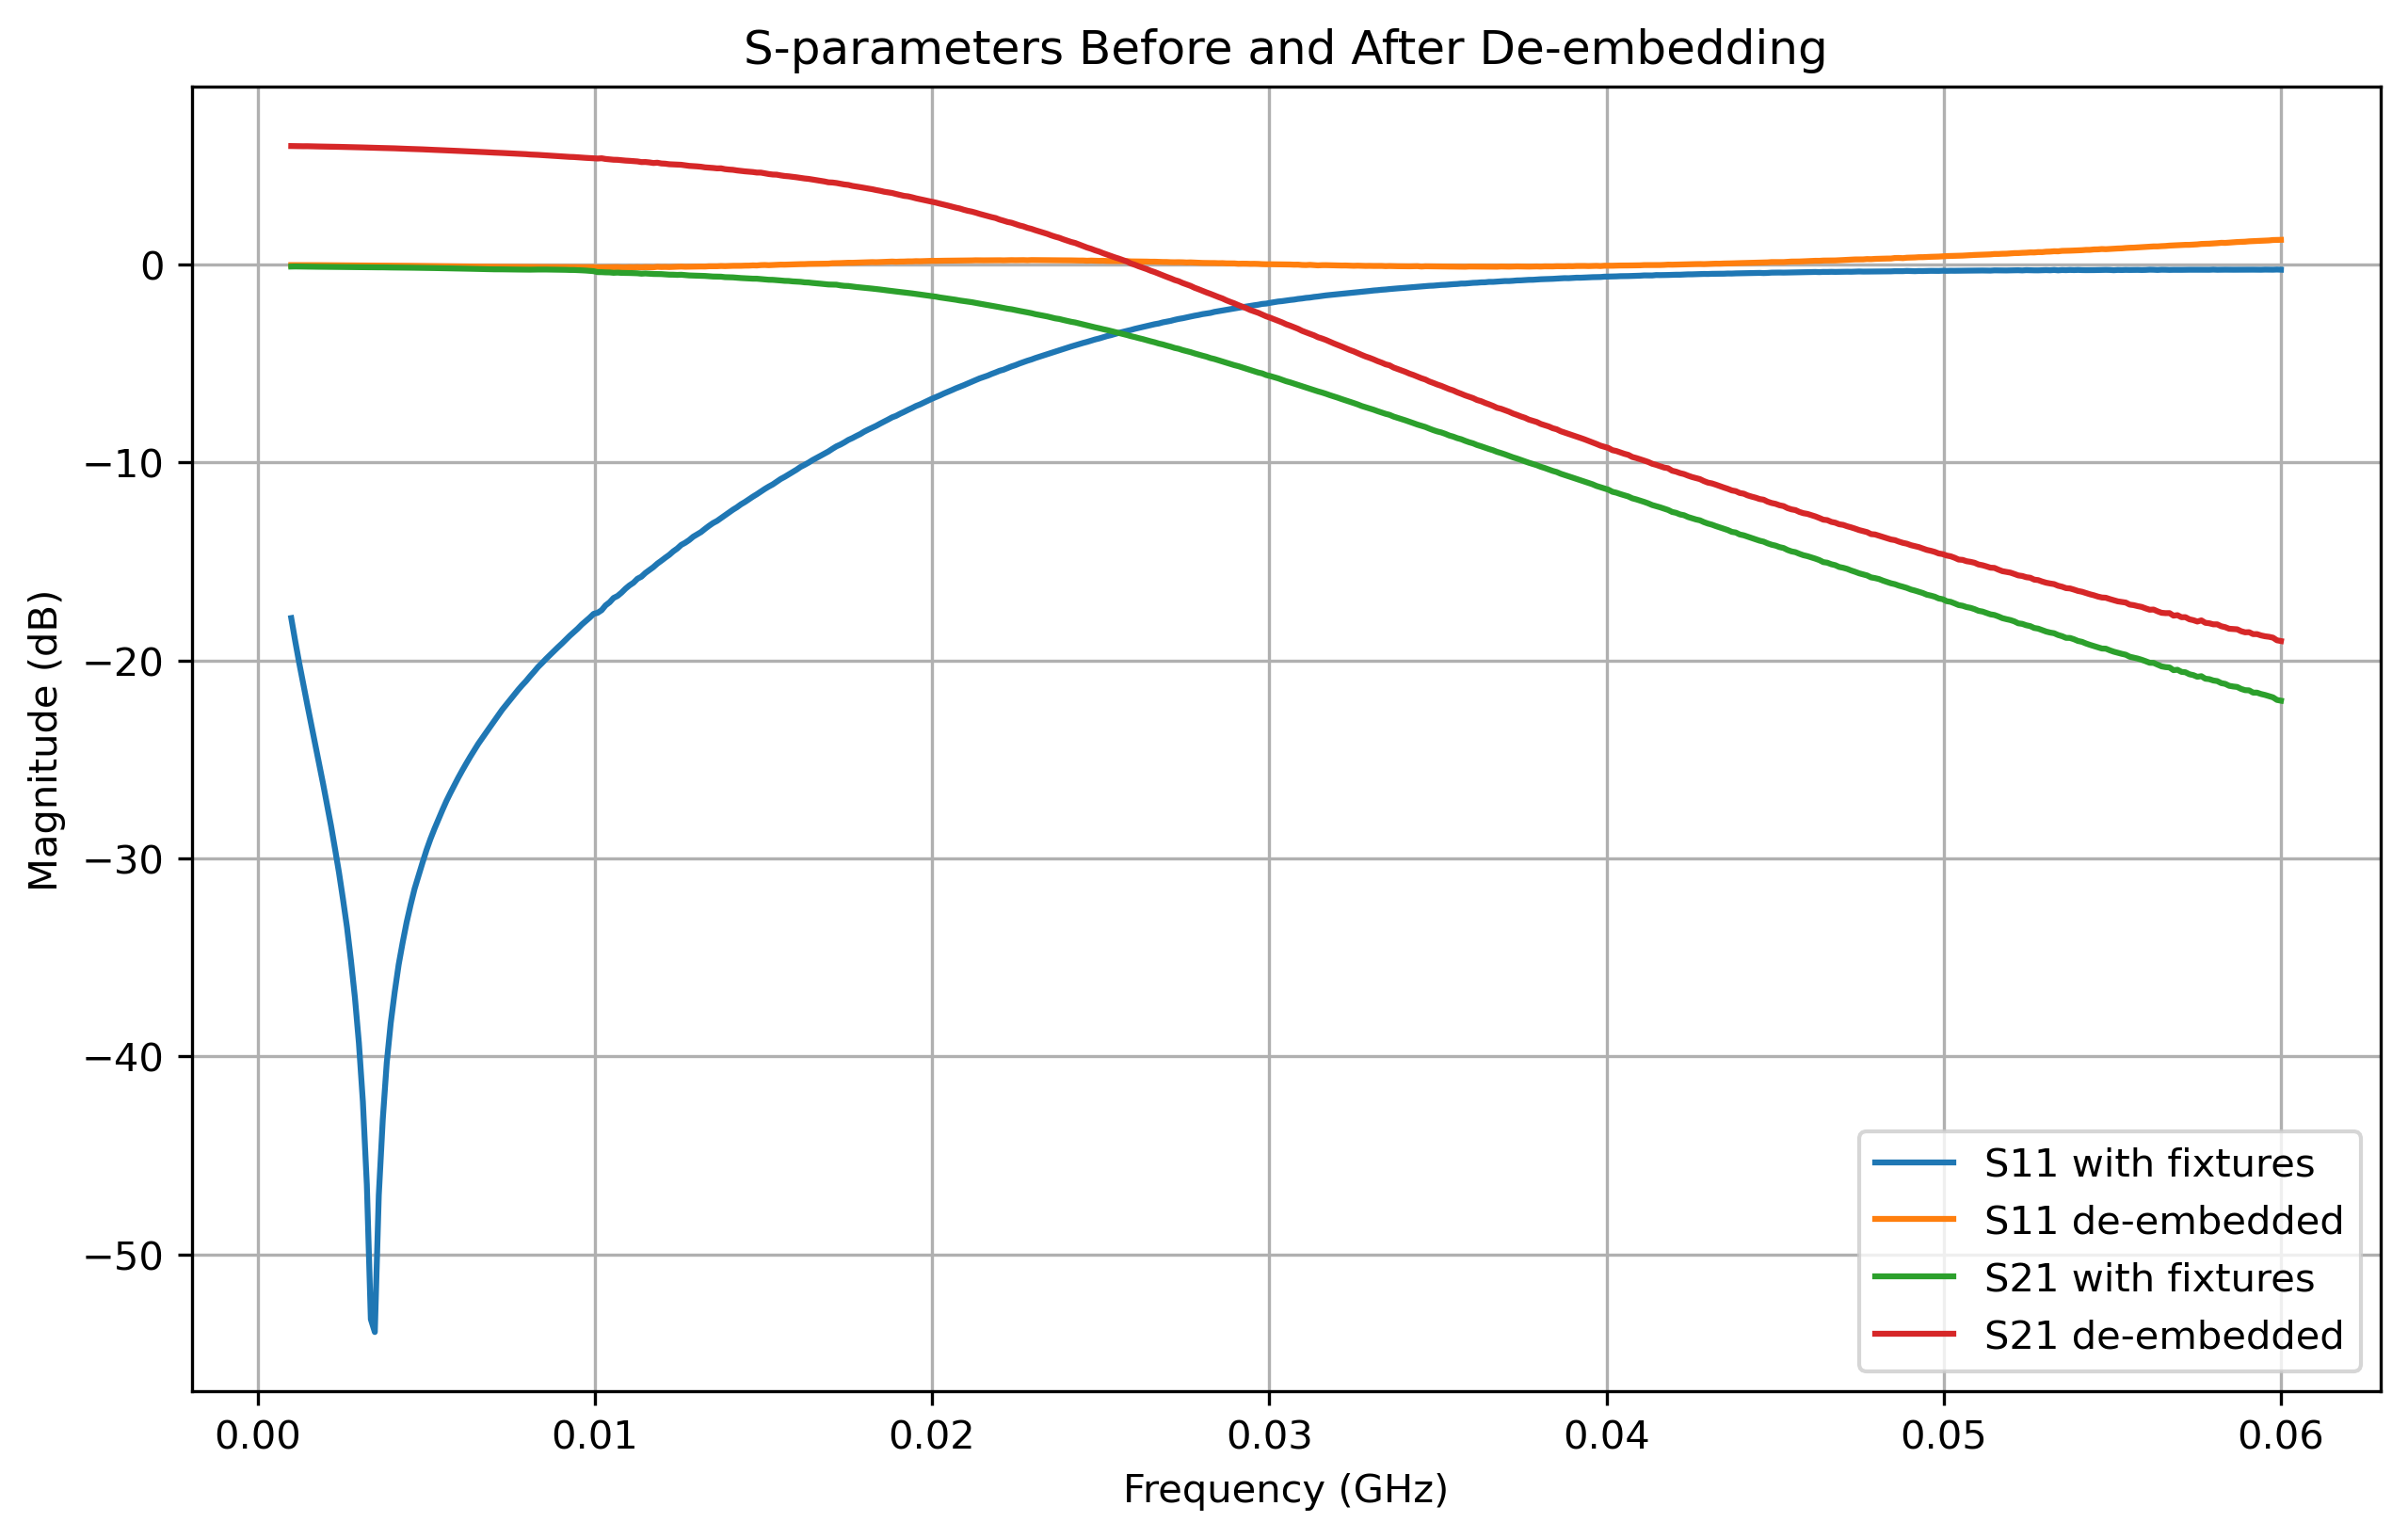
\includegraphics[width=.85\textwidth]{Chapter_8/images/Lab_08_ieee_thru_sparameters_plot.png}
\caption{Plot generated by python code implementing the IEEE thru de-embedding standard. \cite{ieee370_2020}}
\label{Ch8_fig:7}
\end{figure}

% -----------------------------------------------------------------------------
% Figures
% -----------------------------------------------------------------------------
\begin{figure}[H]
\centering
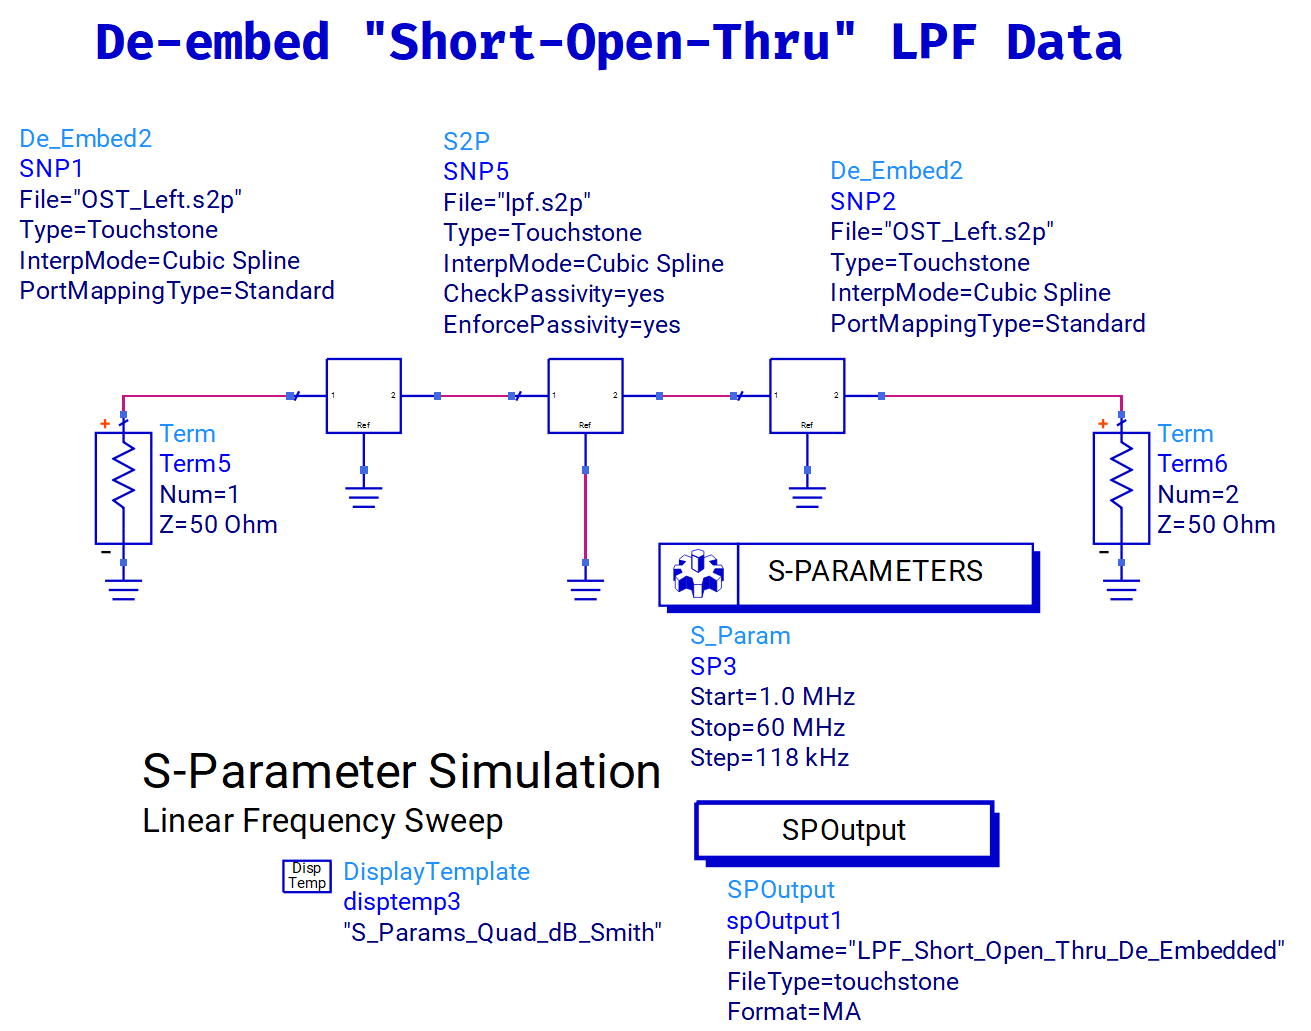
\includegraphics[width=0.9\textwidth]{Chapter_8/images/Lab_08_de-embedded-SOT_Schematic.png}
\caption{ADS schematic implementing OST de-embedding with \texttt{De\_Embed2}. The DUT is the central LPF touchstone block.}
\label{Ch8_fig:8}
\end{figure}

\begin{figure}[H]
\centering
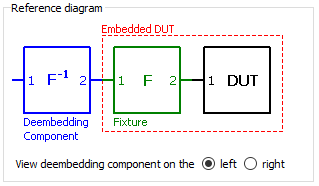
\includegraphics[width=0.6\textwidth]{Chapter_8/images/Lab_08_left-de-embed-reference.png}
\caption{Left-reference positioning used in the ADS \texttt{De\_Embed2} element.}
\label{Ch8_fig:9}
\end{figure}

\begin{figure}[H]
\centering
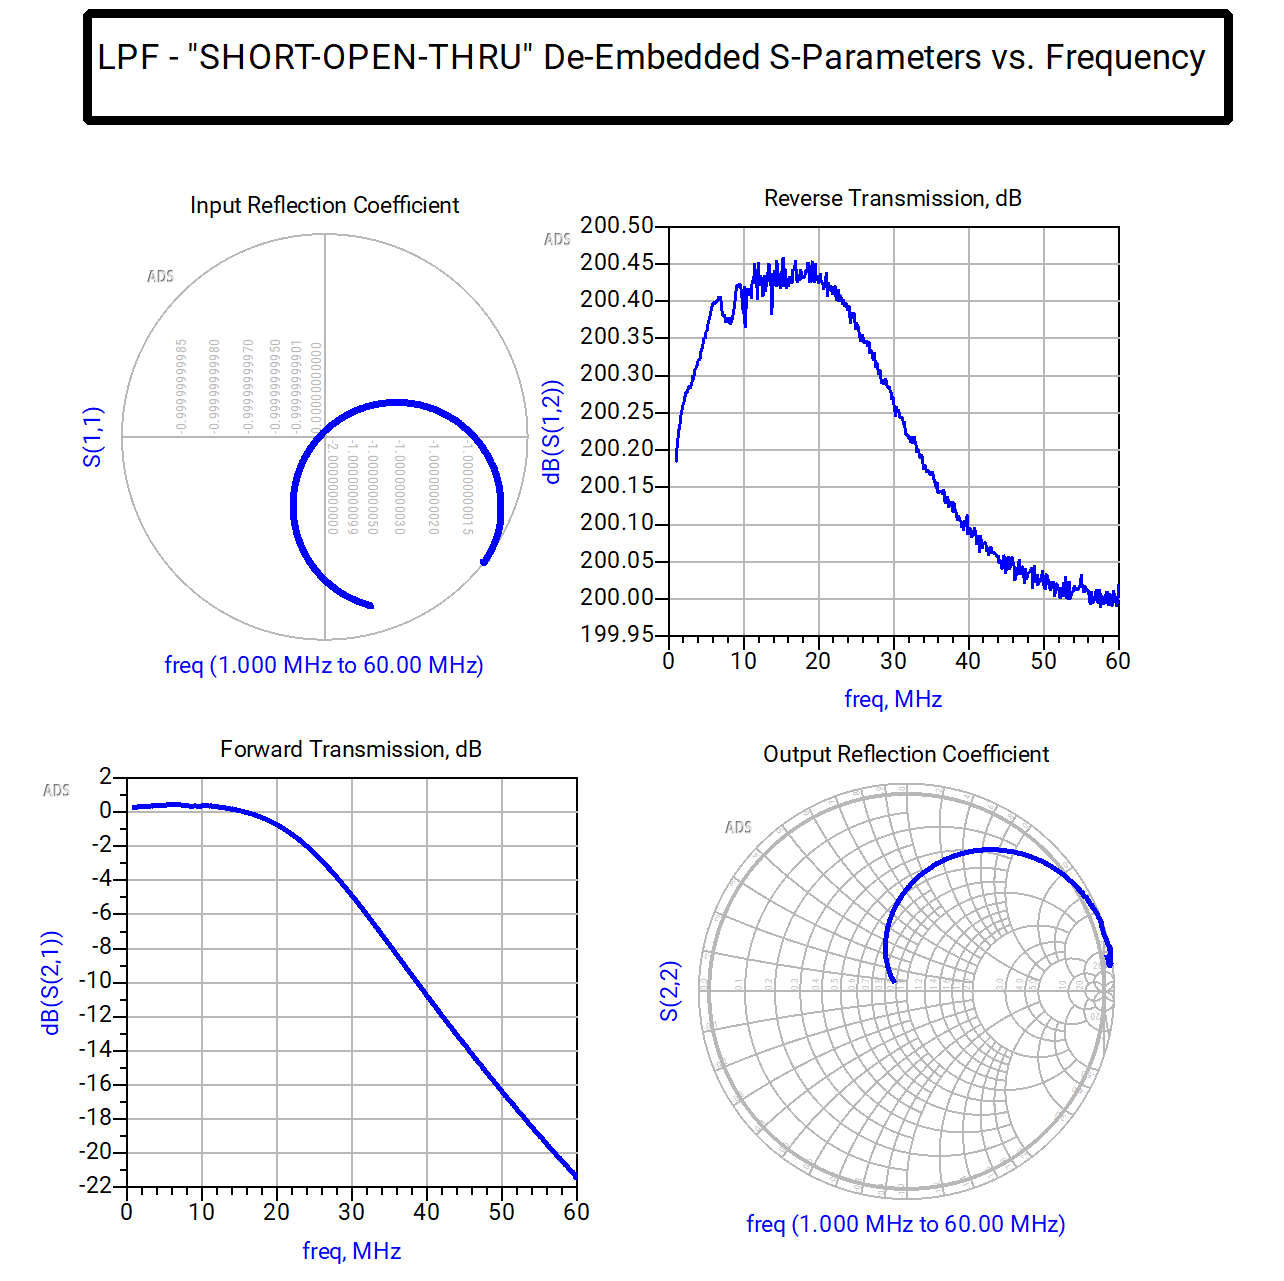
\includegraphics[width=0.9\textwidth]{Chapter_8/images/Lab_08_De-Embedded-SOT_ADS-Plots.png}
\caption{Low-pass filter after OST de-embedding: ADS simulation. Compare with Fig.~\ref{Ch8_fig:5}.}
\label{Ch8_fig:10}
\end{figure}

\begin{figure}[H]
\centering
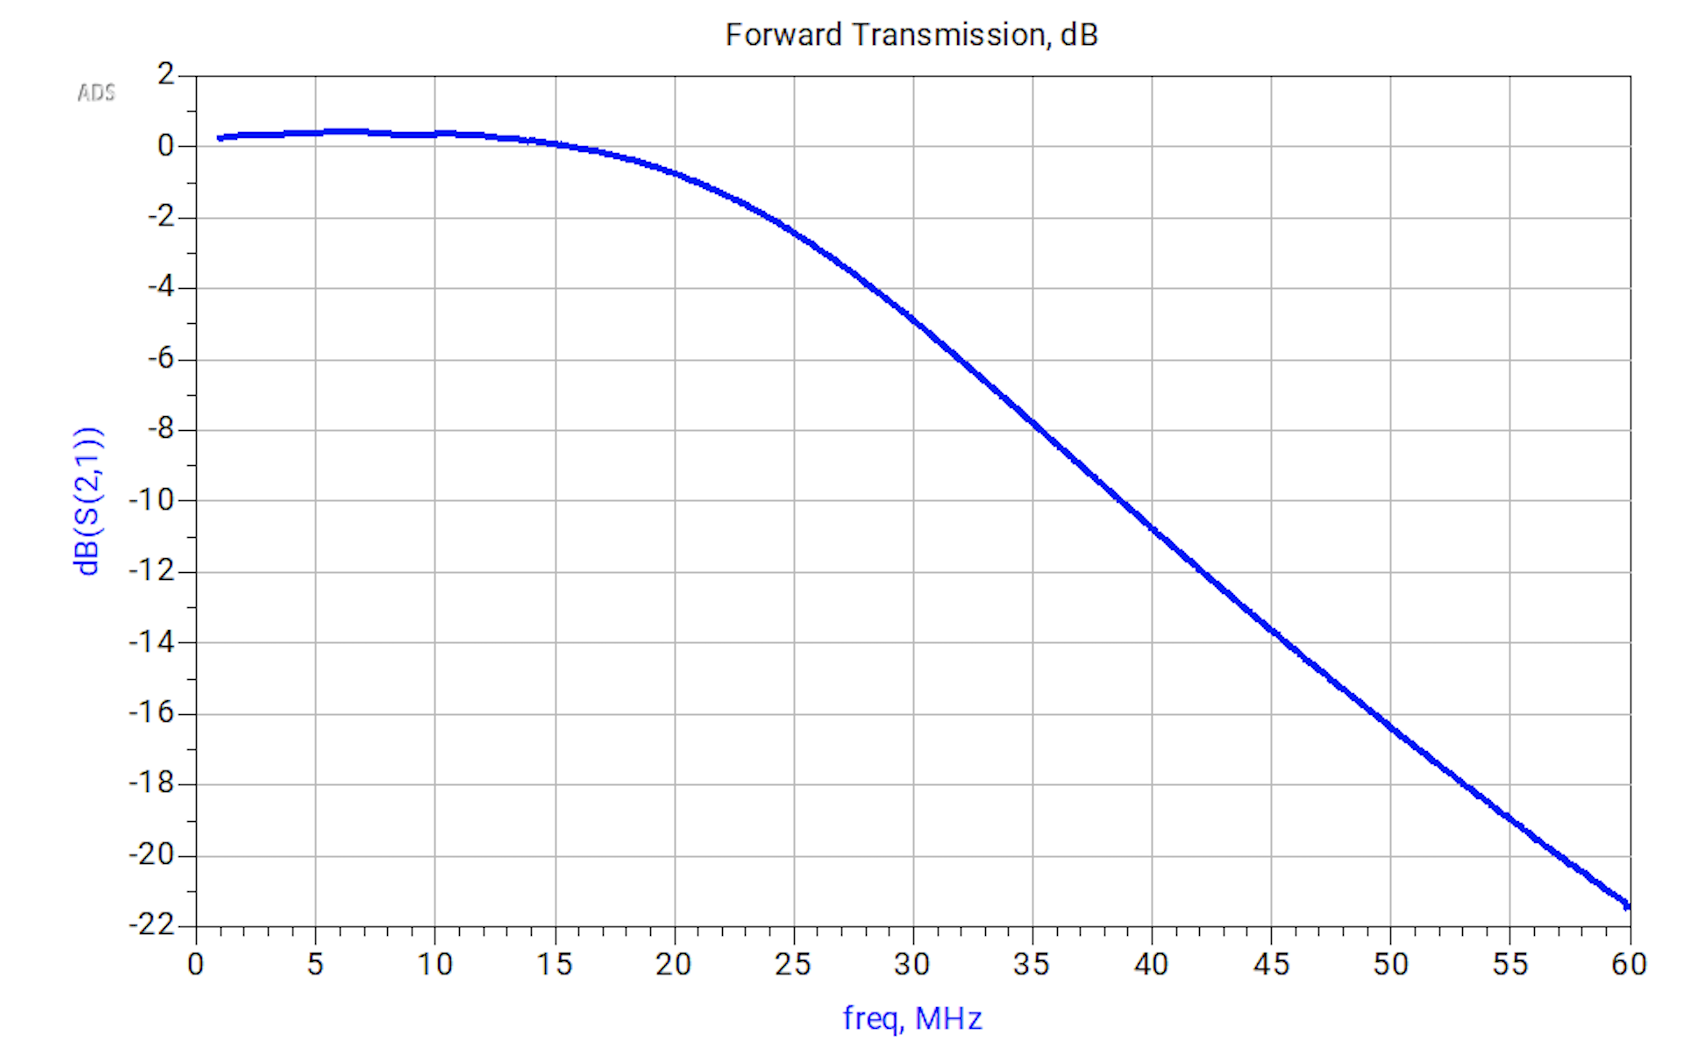
\includegraphics[width=0.875\textwidth]{Chapter_8/images/Lab_08_LPF_OST_S21.png}
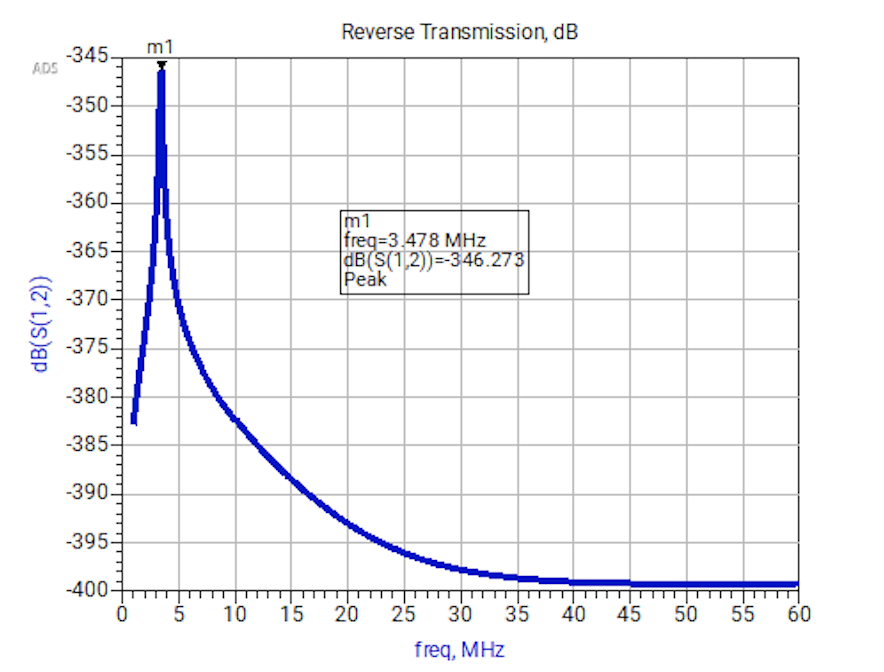
\includegraphics[width=0.875\textwidth]{Chapter_8/images/Lab_08_DeEmbed_Short_2.png}
\caption{Validation of de-embedding on fixture structures.}
\label{Ch8_fig:11}
\end{figure}
\par
The previously un-recognizable curve a low-pass filter response appears after $S-$parameter de-embedding (top). Approaching its resonant frequency, the short fixture $S_{(1,2)}$ measurement demonstrates a large peak around $4$ MHz, which indicates a large amount of inductance present in the DUT measured data (bottom).
\FloatBarrier
\newpage

\section{Python Code Listings}

The Python code for S-parameter de-embedding can be found in the Appendix: LPF Open-Short-Thru Method (\cref{lst:Ch8:List1}), Thru Method (\cref{lst:Ch8:List2}), LPF IEEE Thru Method (\cref{lst:Ch8:List3}), 2x Thru Method (\cref{lst:Ch8:List4}), HPF OST Method (\cref{lst:Ch8:List5}), and HPF IEEE Thru Method (\cref{lst:Ch8:List6}).

\section{Conclusion}

\justifying
\begin{itemize}
\item Practical experience was gained in the setup and calibration of a Vector Network Analyzer (VNA), including the application of Short-Open-Load-Thru (SOLT) calibration standards.
\item The physical significance of scattering parameters, particularly \(S_{21}\) (forward transmission) and \(S_{11}\) (input reflection), was investigated and analyzed.
\item The frequency responses of low-pass and high-pass filters were measured, with key characteristics such as cutoff frequencies and stop-band attenuation identified.
\item Industry-standard de-embedding techniques were applied to isolate the intrinsic behavior of the device under test (DUT) from parasitic effects introduced by the measurement fixtures.
\item The effects of de-embedding on the measured data were analyzed to highlight the importance of fixture error correction in high-frequency characterization.
\item Best practices in RF measurement procedures were reinforced, and the practical application of network theory concepts was demonstrated through experimental verification.
\end{itemize}

\begin{center}
\begin{figure}[H]
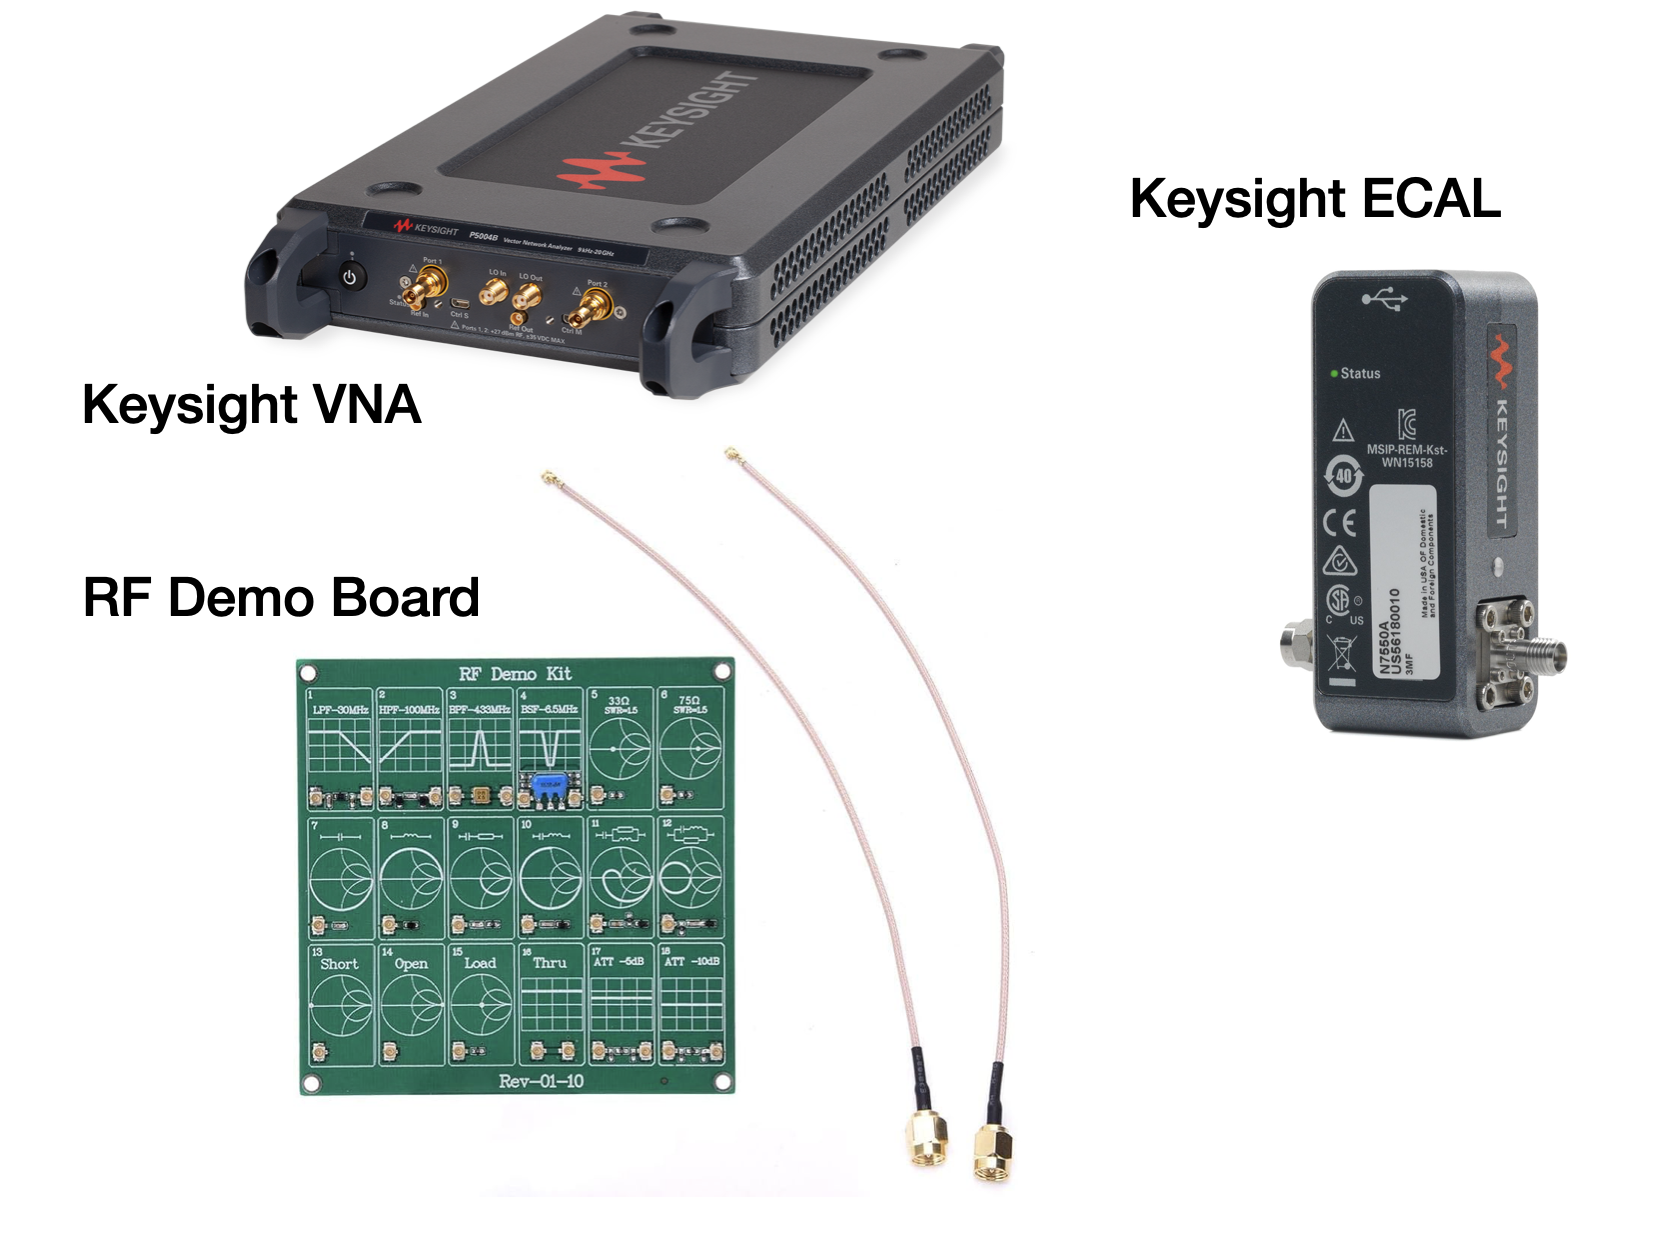
\includegraphics[scale=0.5]{Chapter_8/images/Lab_08_Image_1.png}
\caption{Components utilized during Lab 08 including the Keysight VNA, ECAL calibration module, and RF Demo Board under test}
\label{Ch8_fig:12}
\end{figure}
\end{center}

\clearpage
\printbibliography[heading=subbibliography]